\section{Vurdering}
På bagrund af graferne i sektion \ref{ch4_design} kan det vurderes, at det designede FIR-filter formår at filtrere frekvensen $\omega_2=\frac{\pi}{2}$ fra det samplede signal $s[n]$ som ønsket ved anvendelse af orden større end $30$. \\
Figur \ref{fig:filter_rekt} illustrerer, at de opstillede specifikationer til en vis grad overholdes ved en orden på henholdsvis 30 og 100 og anvendelse af det rektangulære vindue. Det ses tydeligt, at transitionsbåndet bliver smallere og at stopbåndet flader ud jo højere orden der anvendes. De ripples, der forekommer i pasbåndet formindskes også, når ordenen øges. Dog forsvinder de ikke, da det er det rektangulære vindue, der anvendes. Som nævnt kan dette optimeres ved at ændre på vinduet. Herunder optimeres filteret.

\section{Optimering}
Ud fra ovenstående forsøges der med højere filterorden. Forsøg har vist, at der opnås en god filtrering ved hjælp af Hamming-vinduet med $M=92$, hvormed frekvensen $\omega_2 = \pi/2$ filtreres fra uden at påvirke de øvrige frekvenser i udstrakt grad. Dette resultat ses på figur \ref{fig:resultat_freq}, der viser frekvensspektret, hvor frekvensen $\omega_2$ ikke fremgår \todo{Der er lidt rod med enhederne mellem figurerne i kapitel 3 og 4... \textregistered}, og figur \ref{fig:resultat_signal}, der viser det ideelle filtrerede signal plottet oveni det filtrerede signal. Af sidstnævnte fremgår det, at de to signaler ligger oveni hinanden med enkelte afvigelser.
\begin{figure}[H]
\begin{minipage}{0.49\textwidth}
\centering
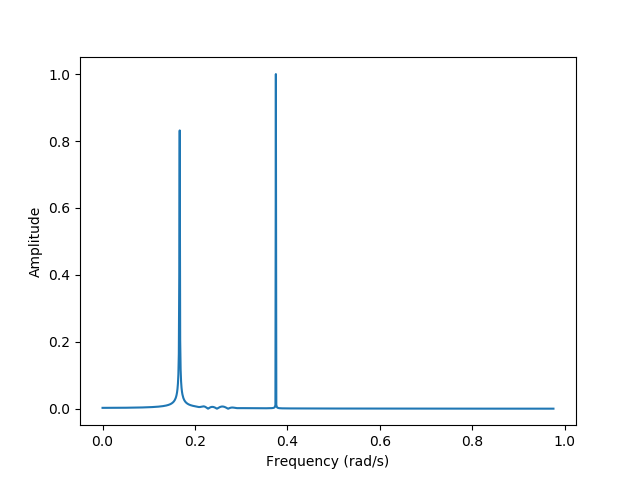
\includegraphics[width=\textwidth]{figures/sf1.png}
\caption{Frekvensspektrum for det filtrerede signal under anvendelse af filter af orden $M=92$.}
\label{fig:resultat_freq}
\end{minipage}
\begin{minipage}{0.49\textwidth}
\centering
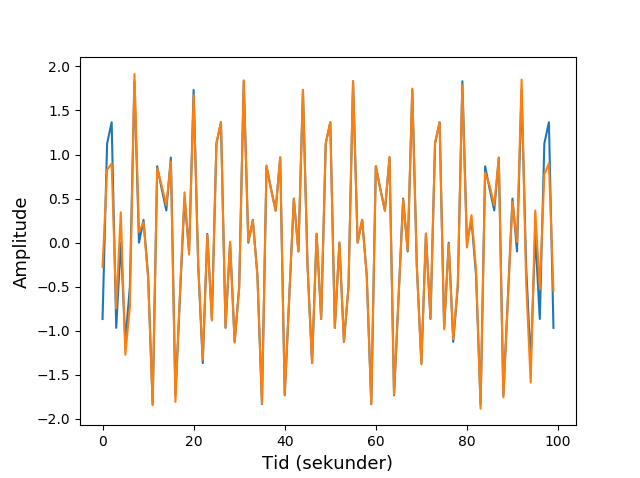
\includegraphics[width=\textwidth]{figures/sf.png}
\caption{Det ideelle filtrerede signal (blå) og det filtrerede signal (orange) samplet ved 1 Hz.}
\label{fig:resultat_signal}
\end{minipage}
\end{figure}

Amplituderesponsen i dB for Hammingvinduet brugt til filteret ses desuden på figur \ref{fig:amplituderespons} i bilag \ref{app2} \todo{Er det vigtigt? \textregistered}.